% Bab IV  Hasil dan Pembahasan
\chapter{HASIL DAN PEMBAHASAN}

\section{Hasil Penelitian}
Hasil penelitian berisi data primer dan atau sekunder. Hasil kuantitatif disajikan dalam bentuk tabel, grafik, dan foto, dan sebaiknya berupa hasil olahan, bukan data mentah. Narasi hasil memuat ulasan makna dari tabel dan gambar, misalnya Tabel 4.1 dan Gambar 4.1 (bab 4, urutan pertama).

\subsection{Hasil Implementasi}
Uraikan hasil implementasi sistem.

\subsection{Hasil Pengujian}
Sajikan hasil pengujian sesuai indikator kinerja pada Bab III.

\begin{singlespace}
\begin{longtable}{|p{0.32\linewidth}|p{0.28\linewidth}|p{0.28\linewidth}|}
\caption{Contoh tabel hasil pengujian}\\
\hline
\textbf{Parameter} & \textbf{Hasil} & \textbf{Keterangan} \\
\hline
Parameter 1 & 0,00 & Keterangan 1 \\
\hline
Parameter 2 & 0,00 & Keterangan 2 \\
\hline
Parameter 3 & 0,00 & Keterangan 3 \\
\hline

\end{longtable}
\end{singlespace}

\begin{figure}[H]
\centering
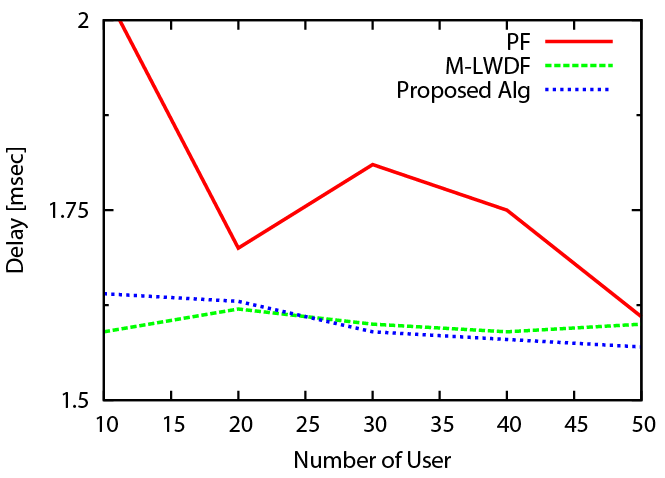
\includegraphics[width=0.6\textwidth]{../gambar/contoh-grafik-warna.png}
\caption{Contoh grafik hasil penelitian}
\end{figure}

\section{Pembahasan}
Pembahasan dikemukakan secara komprehensif, dikaitkan dengan hasil penelitian lain dan teori pada Bab II, baik secara kualitatif maupun kuantitatif.

\textit{Contoh kalimat bersitasi:} Hasil penelitian ini sejalan dengan temuan Capozzi et al. (2013) bahwa …, tetapi berbeda dengan hasil Xu dan Fischione (2012) yang …
